% Options for packages loaded elsewhere
\PassOptionsToPackage{unicode}{hyperref}
\PassOptionsToPackage{hyphens}{url}
\documentclass[
  ignorenonframetext,
]{beamer}
\newif\ifbibliography
\usepackage{pgfpages}
\setbeamertemplate{caption}[numbered]
\setbeamertemplate{caption label separator}{: }
\setbeamercolor{caption name}{fg=normal text.fg}
\beamertemplatenavigationsymbolsempty
% remove section numbering
\setbeamertemplate{part page}{
  \centering
  \begin{beamercolorbox}[sep=16pt,center]{part title}
    \usebeamerfont{part title}\insertpart\par
  \end{beamercolorbox}
}
\setbeamertemplate{section page}{
  \centering
  \begin{beamercolorbox}[sep=12pt,center]{section title}
    \usebeamerfont{section title}\insertsection\par
  \end{beamercolorbox}
}
\setbeamertemplate{subsection page}{
  \centering
  \begin{beamercolorbox}[sep=8pt,center]{subsection title}
    \usebeamerfont{subsection title}\insertsubsection\par
  \end{beamercolorbox}
}
% Prevent slide breaks in the middle of a paragraph
\widowpenalties 1 10000
\raggedbottom
\AtBeginPart{
  \frame{\partpage}
}
\AtBeginSection{
  \ifbibliography
  \else
    \frame{\sectionpage}
  \fi
}
\AtBeginSubsection{
  \frame{\subsectionpage}
}
\usepackage{iftex}
\ifPDFTeX
  \usepackage[T1]{fontenc}
  \usepackage[utf8]{inputenc}
  \usepackage{textcomp} % provide euro and other symbols
\else % if luatex or xetex
  \usepackage{unicode-math} % this also loads fontspec
  \defaultfontfeatures{Scale=MatchLowercase}
  \defaultfontfeatures[\rmfamily]{Ligatures=TeX,Scale=1}
\fi
\usepackage{lmodern}
\ifPDFTeX\else
  % xetex/luatex font selection
\fi
% Use upquote if available, for straight quotes in verbatim environments
\IfFileExists{upquote.sty}{\usepackage{upquote}}{}
\IfFileExists{microtype.sty}{% use microtype if available
  \usepackage[]{microtype}
  \UseMicrotypeSet[protrusion]{basicmath} % disable protrusion for tt fonts
}{}
\makeatletter
\@ifundefined{KOMAClassName}{% if non-KOMA class
  \IfFileExists{parskip.sty}{%
    \usepackage{parskip}
  }{% else
    \setlength{\parindent}{0pt}
    \setlength{\parskip}{6pt plus 2pt minus 1pt}}
}{% if KOMA class
  \KOMAoptions{parskip=half}}
\makeatother
\usepackage{color}
\usepackage{fancyvrb}
\newcommand{\VerbBar}{|}
\newcommand{\VERB}{\Verb[commandchars=\\\{\}]}
\DefineVerbatimEnvironment{Highlighting}{Verbatim}{commandchars=\\\{\}}
% Add ',fontsize=\small' for more characters per line
\newenvironment{Shaded}{}{}
\newcommand{\AlertTok}[1]{\textcolor[rgb]{1.00,0.00,0.00}{\textbf{#1}}}
\newcommand{\AnnotationTok}[1]{\textcolor[rgb]{0.38,0.63,0.69}{\textbf{\textit{#1}}}}
\newcommand{\AttributeTok}[1]{\textcolor[rgb]{0.49,0.56,0.16}{#1}}
\newcommand{\BaseNTok}[1]{\textcolor[rgb]{0.25,0.63,0.44}{#1}}
\newcommand{\BuiltInTok}[1]{\textcolor[rgb]{0.00,0.50,0.00}{#1}}
\newcommand{\CharTok}[1]{\textcolor[rgb]{0.25,0.44,0.63}{#1}}
\newcommand{\CommentTok}[1]{\textcolor[rgb]{0.38,0.63,0.69}{\textit{#1}}}
\newcommand{\CommentVarTok}[1]{\textcolor[rgb]{0.38,0.63,0.69}{\textbf{\textit{#1}}}}
\newcommand{\ConstantTok}[1]{\textcolor[rgb]{0.53,0.00,0.00}{#1}}
\newcommand{\ControlFlowTok}[1]{\textcolor[rgb]{0.00,0.44,0.13}{\textbf{#1}}}
\newcommand{\DataTypeTok}[1]{\textcolor[rgb]{0.56,0.13,0.00}{#1}}
\newcommand{\DecValTok}[1]{\textcolor[rgb]{0.25,0.63,0.44}{#1}}
\newcommand{\DocumentationTok}[1]{\textcolor[rgb]{0.73,0.13,0.13}{\textit{#1}}}
\newcommand{\ErrorTok}[1]{\textcolor[rgb]{1.00,0.00,0.00}{\textbf{#1}}}
\newcommand{\ExtensionTok}[1]{#1}
\newcommand{\FloatTok}[1]{\textcolor[rgb]{0.25,0.63,0.44}{#1}}
\newcommand{\FunctionTok}[1]{\textcolor[rgb]{0.02,0.16,0.49}{#1}}
\newcommand{\ImportTok}[1]{\textcolor[rgb]{0.00,0.50,0.00}{\textbf{#1}}}
\newcommand{\InformationTok}[1]{\textcolor[rgb]{0.38,0.63,0.69}{\textbf{\textit{#1}}}}
\newcommand{\KeywordTok}[1]{\textcolor[rgb]{0.00,0.44,0.13}{\textbf{#1}}}
\newcommand{\NormalTok}[1]{#1}
\newcommand{\OperatorTok}[1]{\textcolor[rgb]{0.40,0.40,0.40}{#1}}
\newcommand{\OtherTok}[1]{\textcolor[rgb]{0.00,0.44,0.13}{#1}}
\newcommand{\PreprocessorTok}[1]{\textcolor[rgb]{0.74,0.48,0.00}{#1}}
\newcommand{\RegionMarkerTok}[1]{#1}
\newcommand{\SpecialCharTok}[1]{\textcolor[rgb]{0.25,0.44,0.63}{#1}}
\newcommand{\SpecialStringTok}[1]{\textcolor[rgb]{0.73,0.40,0.53}{#1}}
\newcommand{\StringTok}[1]{\textcolor[rgb]{0.25,0.44,0.63}{#1}}
\newcommand{\VariableTok}[1]{\textcolor[rgb]{0.10,0.09,0.49}{#1}}
\newcommand{\VerbatimStringTok}[1]{\textcolor[rgb]{0.25,0.44,0.63}{#1}}
\newcommand{\WarningTok}[1]{\textcolor[rgb]{0.38,0.63,0.69}{\textbf{\textit{#1}}}}
\usepackage{graphicx}
\makeatletter
\newsavebox\pandoc@box
\newcommand*\pandocbounded[1]{% scales image to fit in text height/width
  \sbox\pandoc@box{#1}%
  \Gscale@div\@tempa{\textheight}{\dimexpr\ht\pandoc@box+\dp\pandoc@box\relax}%
  \Gscale@div\@tempb{\linewidth}{\wd\pandoc@box}%
  \ifdim\@tempb\p@<\@tempa\p@\let\@tempa\@tempb\fi% select the smaller of both
  \ifdim\@tempa\p@<\p@\scalebox{\@tempa}{\usebox\pandoc@box}%
  \else\usebox{\pandoc@box}%
  \fi%
}
% Set default figure placement to htbp
\def\fps@figure{htbp}
\makeatother
\setlength{\emergencystretch}{3em} % prevent overfull lines
\providecommand{\tightlist}{%
  \setlength{\itemsep}{0pt}\setlength{\parskip}{0pt}}
% Auto-generated by infrastructure/rendering/_pdf_latex_helpers.py::extract_math_font_preamble.
% Minimal header passed to Pandoc via -H so Beamer slides pick up the same math font
% as the combined-PDF path. Adjust the manuscript's preamble.md to change the font globally.
\usepackage{unicode-math}
\setmathfont{latinmodern-math.otf}
\usepackage{bookmark}
\IfFileExists{xurl.sty}{\usepackage{xurl}}{} % add URL line breaks if available
\urlstyle{same}
\hypersetup{
  hidelinks,
  pdfcreator={LaTeX via pandoc}}

\author{\texorpdfstring{}{}}
\date{}

\begin{document}

\section{Beyond the Sentence: State Wires Accumulate Semantic History
Across Discourse}\label{sec:discocirc-discourse}

\begin{frame}[allowframebreaks]{Beyond the Sentence: State Wires
Accumulate Semantic History Across Discourse}
\textbf{Where we are in the argument.}
\autoref{sec:categorical-semantics}--\autoref{sec:compact-closure-complexity}
formalised individual sentences as compact-closed string diagrams and
their complexity as a four-metric summary. This chapter extends
composition \emph{across} sentence boundaries: de Felice--Coecke
DisCoCirc adds persistent entity wires that carry an entity's case-role
history across a discourse, so that a three-sentence discourse traces
Alice's NOM → ACC → NOM trajectory and Bob's ACC → NOM trajectory as
first-class diagrammatic data rather than coreference annotation bolted
on after the fact.
\end{frame}

\begin{frame}[fragile,allowframebreaks]{DisCoCirc State Wires Resolve
Coreference and Role Shifts}
\protect\phantomsection\label{discocirc-state-wires-resolve-coreference-and-role-shifts}
De Felice and Coecke {[}-@defelice2020discourse{]} address this
limitation by formulating \textbf{DisCoCirc} (Distributional
Compositional Circuits). DisCoCirc extends the base categorical
framework, empowering it to dynamically handle discourse-level semantic
structure.

Specifically, DisCoCirc introduces continuous \emph{state wires} that
actively persist across isolated sentence boundaries, continuously
encoding the dynamically evolving states of distinct discourse entities
(e.g., characters, objects, shifting topics). For example, a
multi-sentence sequence like ``Alice chased Bob. He was terrified.'' is
explicitly represented as an integrated geometric circuit where:

\begin{itemize}
\tightlist
\item
  Alice and Bob are wires that persist across both sentences.
\item
  The pronoun ``He'' is resolved by actively connecting its topological
  wire directly to Bob's wire.
\item
  The shifting emotional state ``terrified'' seamlessly updates the
  cumulative state information carried exclusively by Bob's persistent
  wire.
\end{itemize}

De Felice et al. {[}-@defelice2022discocirc{]} subsequently extended
this approach, developing a full-fledged, multi-layered circuit model
built to systematically resolve ambiguity, tangled coreference, and
overarching discourse coherence---all locked within the exact same
continuous categorical formalism. A CCG-based pipeline for generating
discourse circuits from syntactic parse trees has demonstrated that
DisCoCirc can scale to text, dynamically composing sentence-level
diagrams along shared entity wires via an iterative process of
coreference resolution and wire merging {[}-@duneau2021parsing{]}. This
pipeline approach has since been extended to a comparative framework for
evaluating compositional AI model architectures
{[}-@duneau2025comparative{]}, confirming that the DisCoCirc
wire-merging strategy generalizes across model families. Complementary
work on \textbf{DiscoSG} (Discourse Scene Graphs) extends this approach
to multi-sentence image captions, parsing text into scene graphs that
capture cross-sentence coreference relations. \autoref{fig:discourse}
illustrates a multi-sentence discourse diagram where entity wires
persist across sentence boundaries. For case theory, DisCoCirc is
significant because it shows how case-marked argument structure
\emph{composes across discourse}: the nominative subject of one sentence
can become the accusative object of the next, and this transformation is
tracked as a morphism in the discourse category.

\begin{figure}
\centering
\pandocbounded{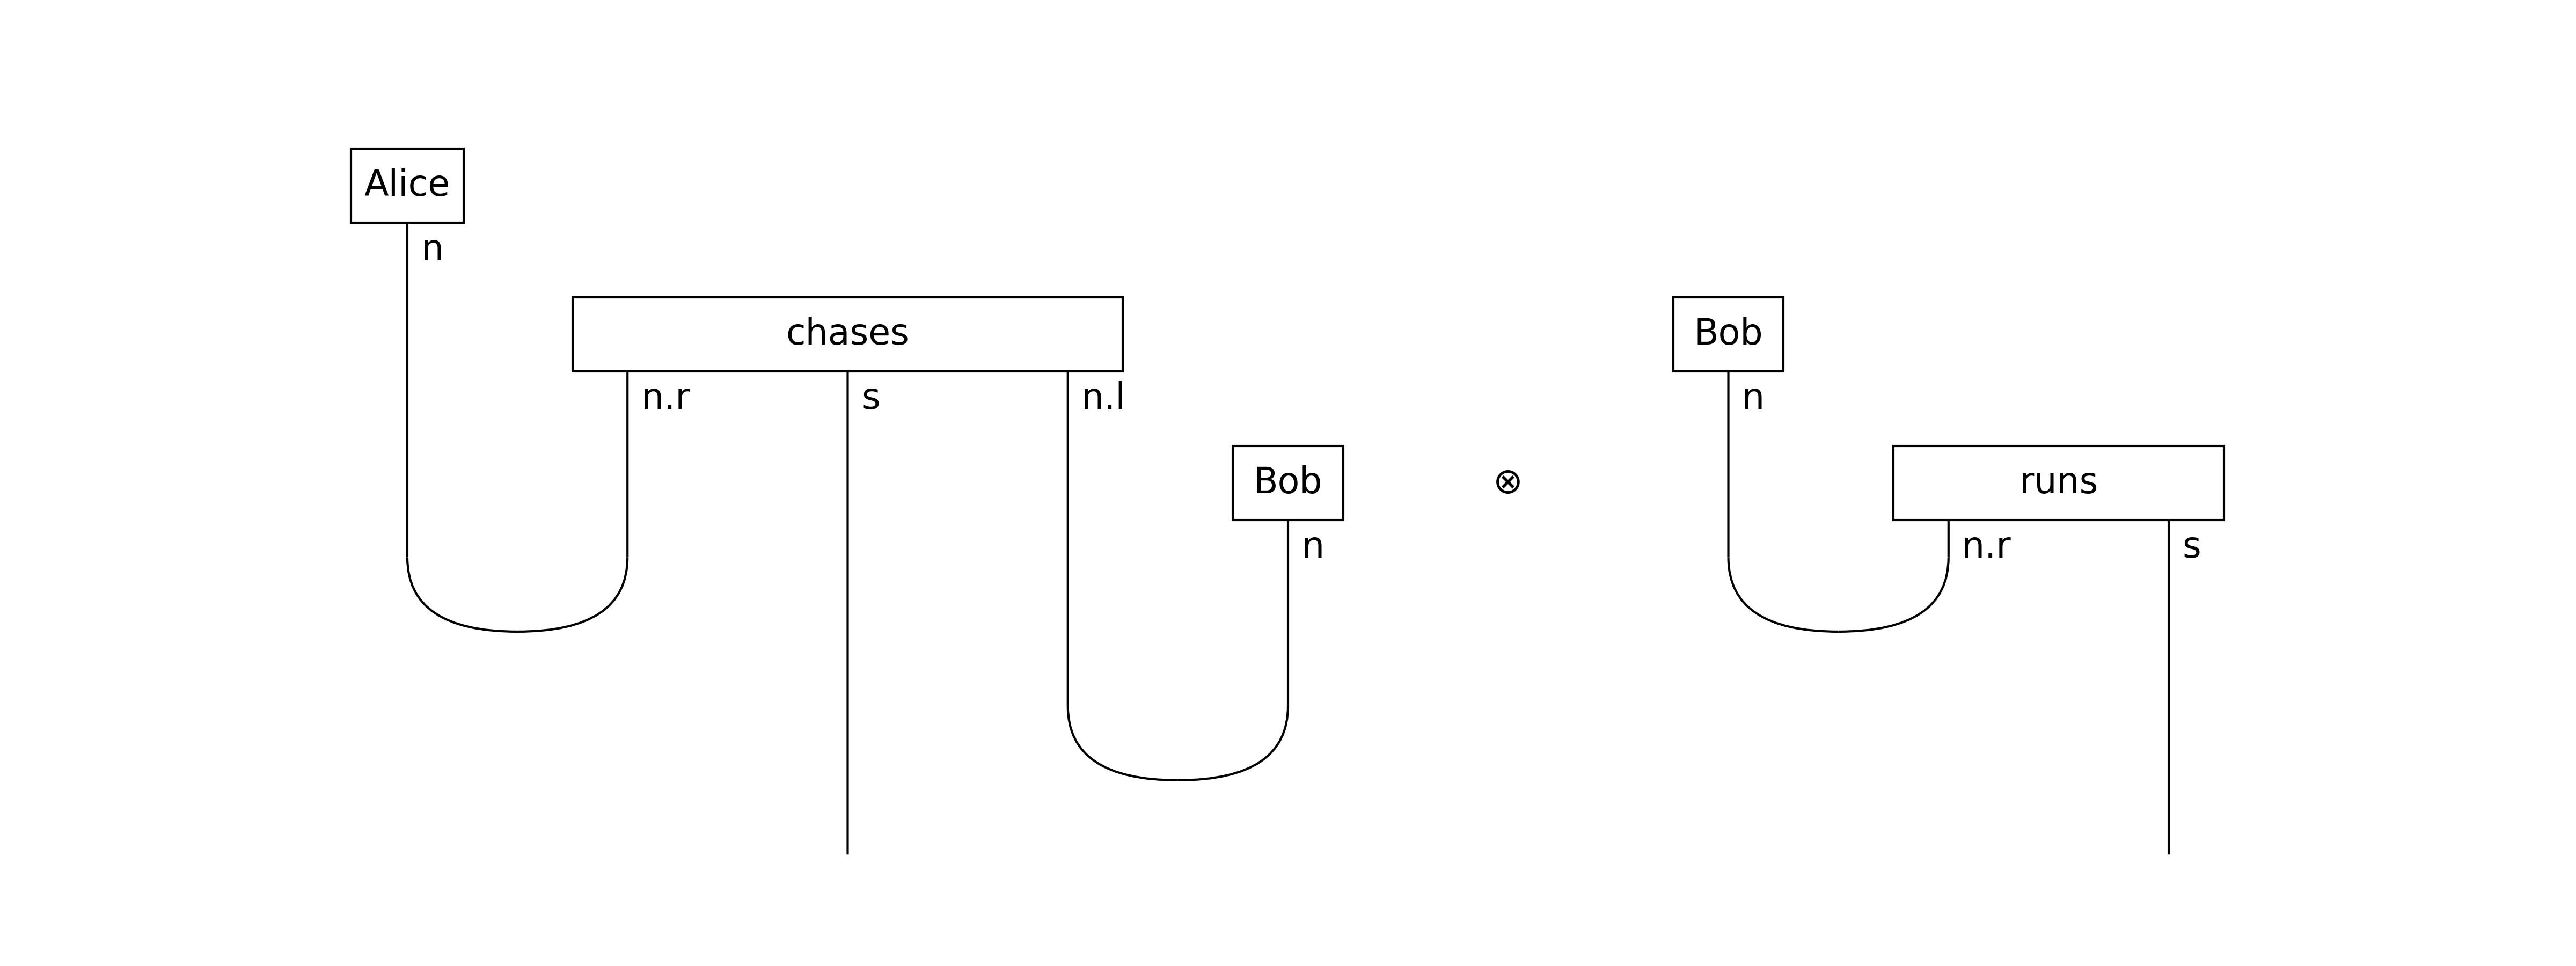
\includegraphics[keepaspectratio,alt={DisCoCirc type structure encodes discourse coherence as a tensor product of sentence types. DisCoPy pregroup grammar for ``Alice chases Bob. Bob runs.'' showing inter-sentential composition. Sentence 1 (left subdiagram): Alice (n) and Bob (n) contract into ``chases'' (n\^{}r \textbackslash otimes s \textbackslash otimes n\^{}l) via two Cups, yielding sentence type s. Sentence 2 (right subdiagram): Bob (n) contracts into ``runs'' (n\^{}r \textbackslash otimes s) via one Cup, yielding s. The joint discourse type s \textbackslash otimes s encodes inter-sentential coherence as a tensor product, the computational primitive that DisCoCirc state wires exploit to propagate Bob's semantic state from ACC (sentence 1) to NOM (sentence 2). See  for wire-colour confirmation of the role transition, and  for the three-sentence DisCoPy tensor layout (role reversal; anaphora is developed in prose and in the Discourse API below, not as a separate pronoun box in the DisCoPy figure).}]{../figures/discopy_discocirc_discourse.png}}
\caption{DisCoCirc type structure encodes discourse coherence as a
tensor product of sentence types. DisCoPy pregroup grammar for ``Alice
chases Bob. Bob runs.'' showing inter-sentential composition.
\textbf{Sentence 1} (left subdiagram): Alice (\(n\)) and Bob (\(n\))
contract into ``chases'' (\(n^r \otimes s \otimes n^l\)) via two Cups,
yielding sentence type \(s\). \textbf{Sentence 2} (right subdiagram):
Bob (\(n\)) contracts into ``runs'' (\(n^r \otimes s\)) via one Cup,
yielding \(s\). The joint discourse type \(s \otimes s\) encodes
inter-sentential coherence as a tensor product, the computational
primitive that DisCoCirc state wires exploit to propagate Bob's semantic
state from ACC (sentence 1) to NOM (sentence 2). See
\autoref{fig:native-discourse} for wire-colour confirmation of the role
transition, and \autoref{fig:three-sentence-discourse} for the
three-sentence DisCoPy tensor layout (role reversal; anaphora is
developed in prose and in the \protect\texttt{Discourse} API below, not
as a separate pronoun box in the DisCoPy figure).}\label{fig:discourse}
\end{figure}

\begin{figure}
\centering
\pandocbounded{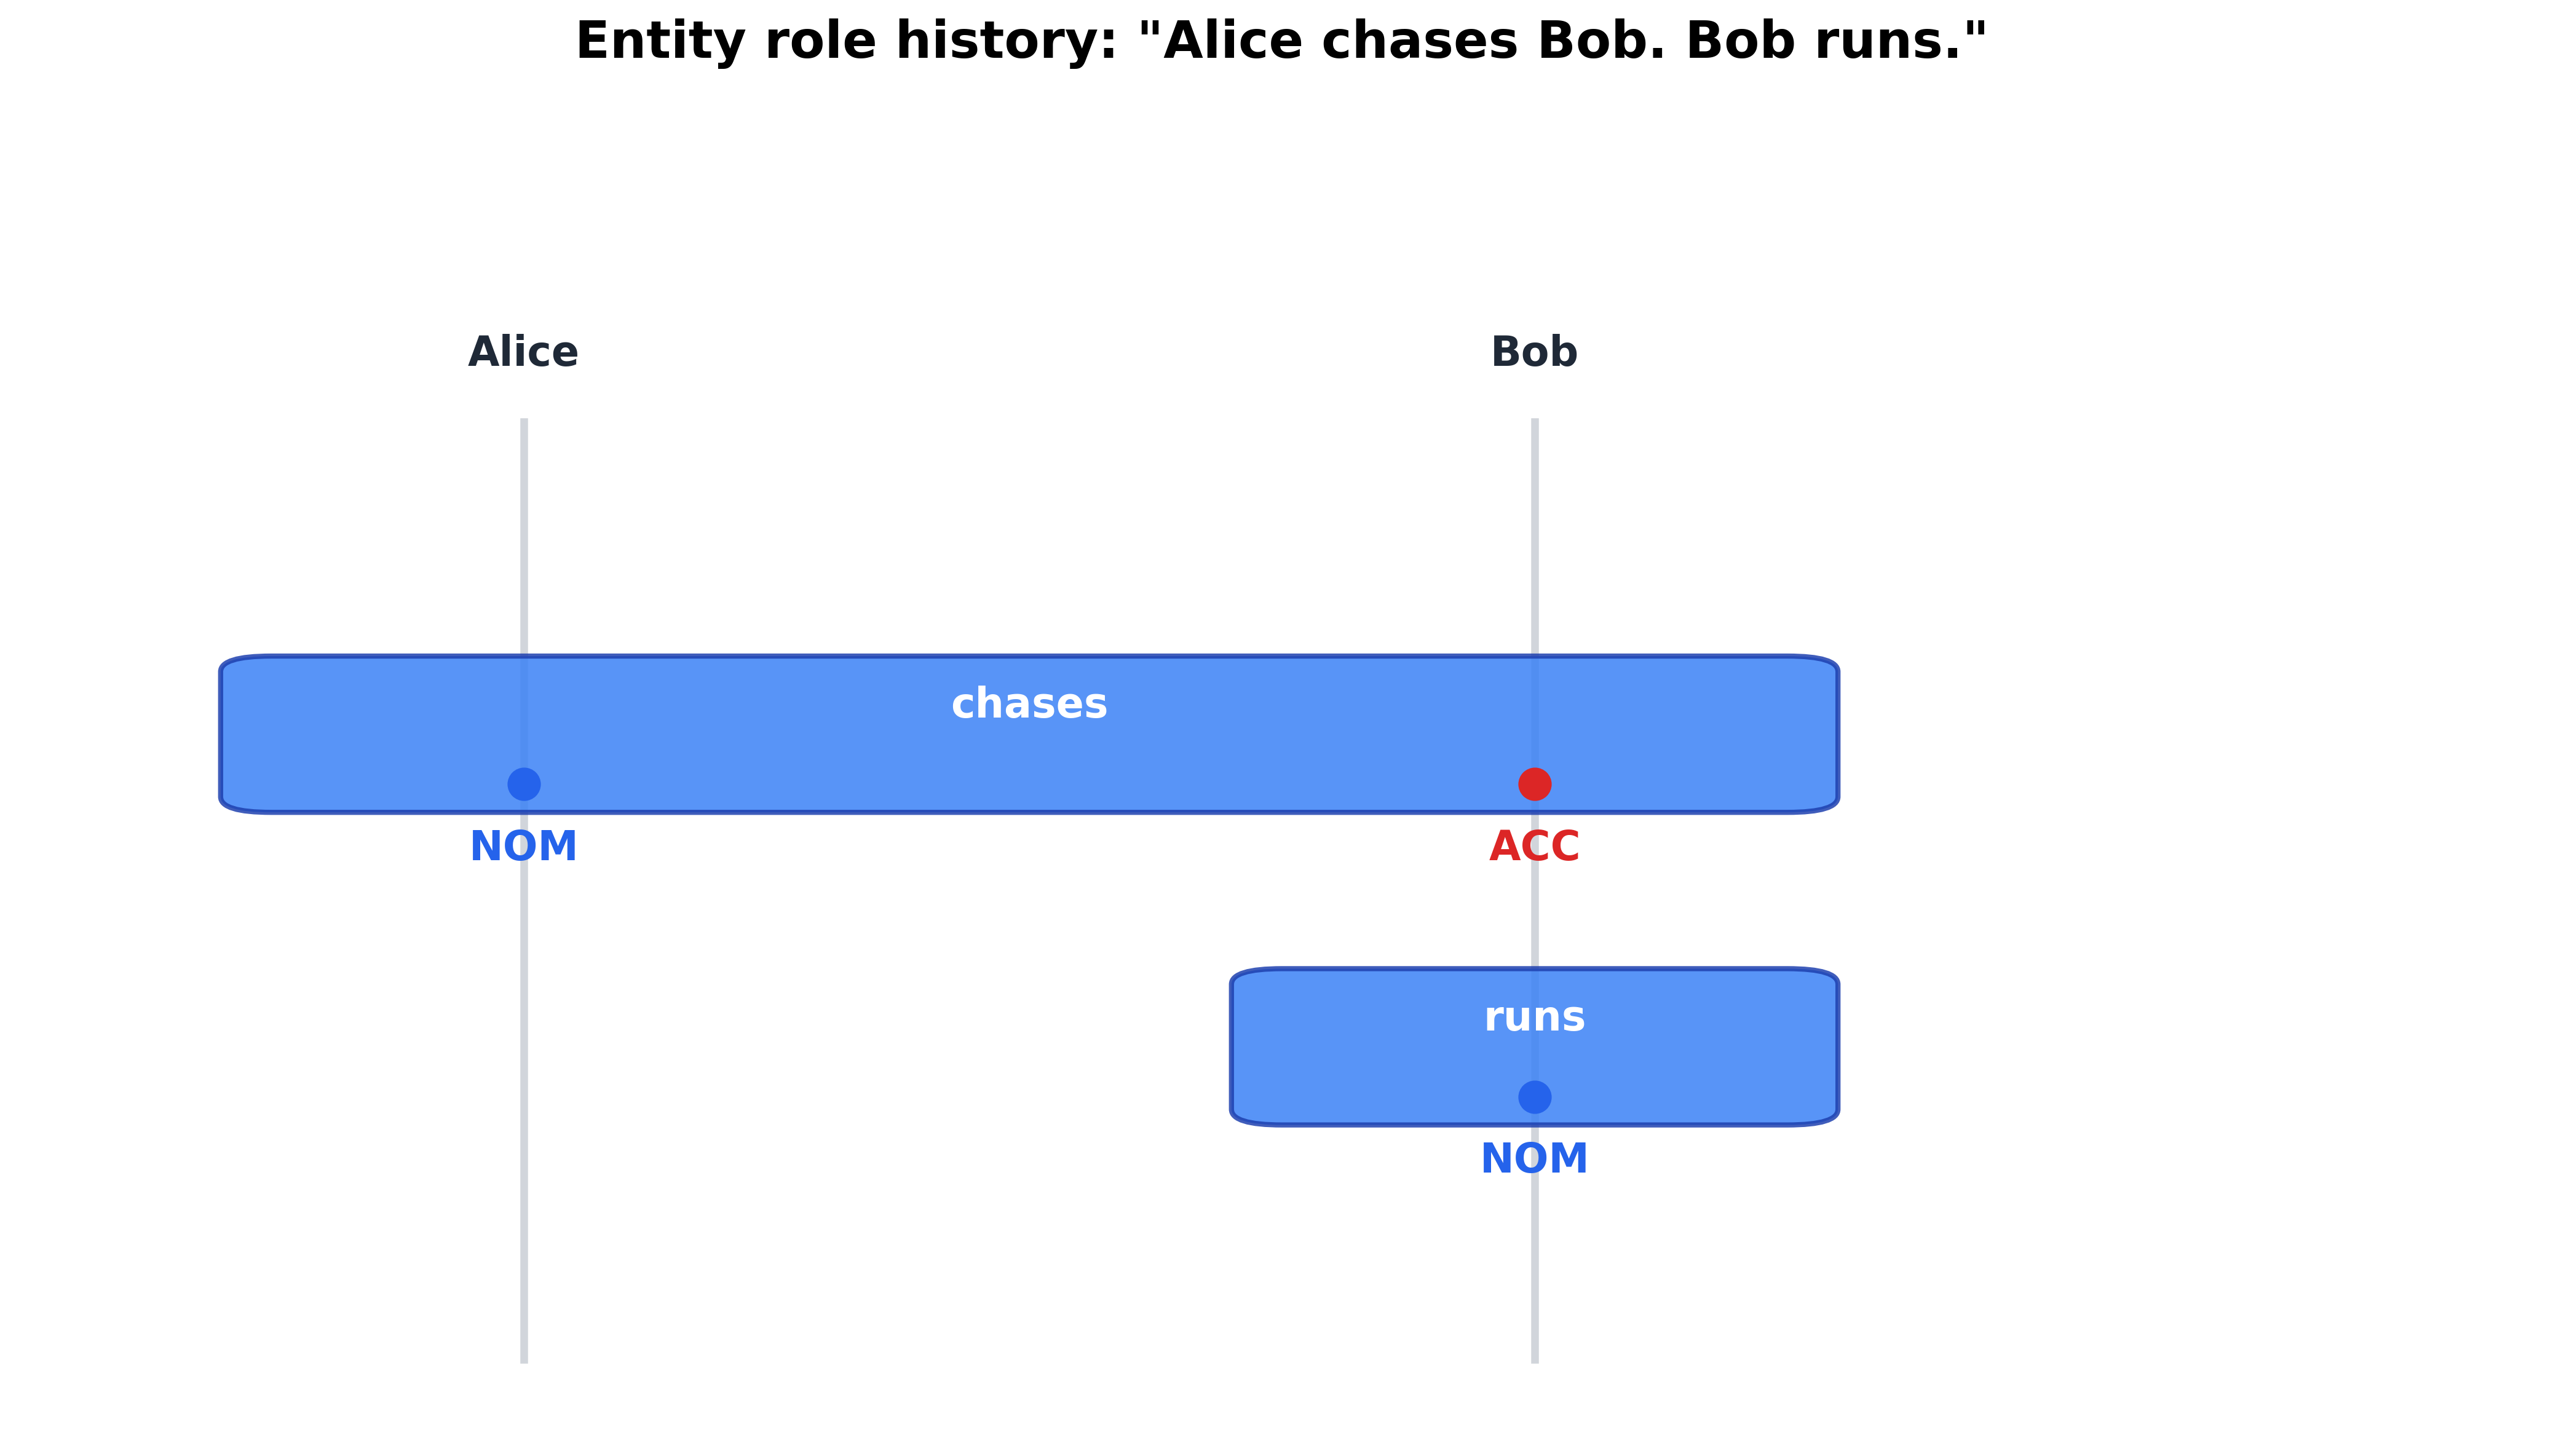
\includegraphics[keepaspectratio,alt={Wire colour provides independent visual confirmation of the ACC\textbackslash toNOM role transition that  encodes algebraically. Native matplotlib DisCoCirc diagram for the same two-sentence discourse, generated via src.visualization.string\_diagrams.render\_discocirc\_discourse() without the DisCoPy library. Vertical grey wires: persistent entity wires for Alice and Bob, confirming that identity is tracked across the sentence boundary. Colour-coded role discs: Bob's wire is marked red (ACC) at sentence 1 (chased object) and blue (NOM) at sentence 2 (running agent). The ACC\textbackslash toNOM colour change is directly readable from the diagram without algebraic computation --- Shimojima's free-ride inference in action. This independent rendering cross-validates that src.diagrams.string\_diagram.Discourse correctly resolves entity identity and role reassignment using only case-role metadata.}]{../figures/discourse_string_diagram.png}}
\caption{Wire colour provides independent visual confirmation of the
ACC\(\to\)NOM role transition that \autoref{fig:discourse} encodes
algebraically. Native matplotlib DisCoCirc diagram for the same
two-sentence discourse, generated via
\protect\texttt{src.visualization.string\_diagrams.render\_discocirc\_discourse()}
without the DisCoPy library. \textbf{Vertical grey wires}: persistent
entity wires for Alice and Bob, confirming that identity is tracked
across the sentence boundary. \textbf{Colour-coded role discs}: Bob's
wire is marked \textbf{red} (ACC) at sentence 1 (chased object) and
\textbf{blue} (NOM) at sentence 2 (running agent). The ACC\(\to\)NOM
colour change is directly readable from the diagram without algebraic
computation --- Shimojima's free-ride inference in action. This
independent rendering cross-validates that
\protect\texttt{src.diagrams.string\_diagram.Discourse} correctly
resolves entity identity and role reassignment using only case-role
metadata.}\label{fig:native-discourse}
\end{figure}
\end{frame}

\begin{frame}[fragile,allowframebreaks]{Alice's Role Trajectory:
NOM→ACC→NOM Across Three Sentences}
\protect\phantomsection\label{alices-role-trajectory-nomaccnom-across-three-sentences}
The power of DisCoCirc for case theory becomes particularly vivid in
multi-sentence discourses where the \emph{same entity occupies different
case roles} across sentences. Consider the three-sentence discourse:

\begin{quote}
\emph{``Alice chases Bob. Bob fears Alice. She smiles.''}
\end{quote}

In this discourse, Alice undergoes a complete cycle of case role
reversals:

\begin{enumerate}
\tightlist
\item
  \textbf{Sentence 1}: Alice is \(\text{NOM}\) (Proto-Agent, the one
  chasing) and Bob is \(\text{ACC}\) (Proto-Patient, the one chased).
\item
  \textbf{Sentence 2}: Bob is now \(\text{NOM}\) (the one fearing) and
  Alice is \(\text{ACC}\) (the one feared)---a role reversal where Alice
  moves from agent to patient.
\item
  \textbf{Sentence 3}: ``She'' resolves anaphorically to Alice, who
  returns to \(\text{NOM}\) as the agent of smiling.
\end{enumerate}

This NOM \(\to\) ACC \(\to\) NOM trajectory for Alice across three
sentences is precisely the kind of \emph{dynamic case assignment} that
static single-sentence analyses cannot capture. The categorical
representation as a triple tensor product \(s \otimes s \otimes s\)
(\autoref{fig:three-sentence-discourse}) encodes each sentence as an
independent pregroup derivation while preserving the entity identity
that links them. This role reversal essentially requires applying the
topological \texttt{Swap} operation (introduced for passivization in
\autoref{sec:case-type-logic}) dynamically across the discourse
boundary. In a full DisCoCirc implementation, Alice's entity wire would
carry accumulated semantic state---the meaning of ``She'' in sentence 3
inherits the enriched state of an Alice who has first chased and then
been feared, not merely the bare lexical entry for ``Alice.''

The trajectory is \emph{executable}: the
\texttt{src.diagrams.string\_diagram.Discourse} class implements exactly
this entity-wire-with-role-history bookkeeping. The following snippet,
taken verbatim from the public API exercised by the test suite, builds
the three-sentence Alice/Bob discourse and reads back the role history
that drives \autoref{fig:three-sentence-discourse}:

\begin{Shaded}
\begin{Highlighting}[]
\ImportTok{from}\NormalTok{ src.diagrams.string\_diagram }\ImportTok{import}\NormalTok{ Sentence, Discourse}

\NormalTok{discourse }\OperatorTok{=}\NormalTok{ Discourse()}
\NormalTok{discourse.add\_sentence(Sentence.transitive(}\StringTok{"Alice"}\NormalTok{, }\StringTok{"chases"}\NormalTok{, }\StringTok{"Bob"}\NormalTok{))}
\NormalTok{discourse.add\_sentence(Sentence.transitive(}\StringTok{"Bob"}\NormalTok{, }\StringTok{"fears"}\NormalTok{, }\StringTok{"Alice"}\NormalTok{))}
\NormalTok{discourse.add\_sentence(Sentence.intransitive(}\StringTok{"Alice"}\NormalTok{, }\StringTok{"smiles"}\NormalTok{))}

\CommentTok{\# Persistent entity wires (DisCoCirc state{-}wire reading)}
\ControlFlowTok{assert}\NormalTok{ discourse.entities }\OperatorTok{==}\NormalTok{ \{}\StringTok{"Alice"}\NormalTok{, }\StringTok{"Bob"}\NormalTok{\}}
\ControlFlowTok{assert}\NormalTok{ discourse.num\_sentences }\OperatorTok{==} \DecValTok{3}

\CommentTok{\# Role history per entity reproduces the NOM → ACC → NOM trajectory}
\ControlFlowTok{assert}\NormalTok{ [r.name }\ControlFlowTok{for}\NormalTok{ r }\KeywordTok{in}\NormalTok{ discourse.role\_history[}\StringTok{"Alice"}\NormalTok{]] }\OperatorTok{==}\NormalTok{ [}\StringTok{"NOM"}\NormalTok{, }\StringTok{"ACC"}\NormalTok{, }\StringTok{"NOM"}\NormalTok{]}
\ControlFlowTok{assert}\NormalTok{ [r.name }\ControlFlowTok{for}\NormalTok{ r }\KeywordTok{in}\NormalTok{ discourse.role\_history[}\StringTok{"Bob"}\NormalTok{]]   }\OperatorTok{==}\NormalTok{ [}\StringTok{"ACC"}\NormalTok{, }\StringTok{"NOM"}\NormalTok{]}

\CommentTok{\# \textasciigrave{}role\_reversal\_entities\textasciigrave{} flags every entity whose case role}
\CommentTok{\# changes across the discourse — the formal analogue of the}
\CommentTok{\# trajectory pictured in \textbackslash{}autoref\{fig:three{-}sentence{-}discourse\}.}
\ControlFlowTok{assert} \BuiltInTok{set}\NormalTok{(discourse.role\_reversal\_entities()) }\OperatorTok{==}\NormalTok{ \{}\StringTok{"Alice"}\NormalTok{, }\StringTok{"Bob"}\NormalTok{\}}
\end{Highlighting}
\end{Shaded}

Slavic discourse supplies a \emph{morphologically overt} analogue of the
persistent state wire: in Serbian/BCS, second-position clitics
(Wackernagel position) such as \emph{je} AUX.3SG, \emph{mu} DAT.3SG.M,
\emph{ga} ACC.3SG.M form a fixed-order cluster that \emph{carries the
case role of the discourse referent forward in time}. \emph{Marko ga je
video} ``Marko him.ACC AUX saw'' and \emph{Dao mu ga je} ``He gave
him.DAT it.ACC AUX'' make Bob's wire-and-case-history visible in the
surface string in a way that English pronouns (which collapse case
morphology onto a tiny three-form \texttt{I/me/my} paradigm) cannot.
Russian, which lacks the BCS clitic cluster, instead encodes the same
persistence directly in the suffix on the noun or full pronoun
(\emph{ego} ACC, \emph{emu} DAT, \emph{im} INS), so role reversals like
Alice's NOM\(\to\)ACC\(\to\)NOM trajectory in \emph{Alisa gonyaet Boba.
Bob boitsja Alisy. Ona ulybaetsja} are reconstructible \emph{from the
morphology alone}, with no positional ambiguity. These are the cleanest
natural-language witnesses for the entity-wire-with-role-history
bookkeeping that the \texttt{Discourse} API formalises.

The point of including the snippet in prose is reproducibility, not
novelty: every assertion above is exercised in
\texttt{tests/test\_diagrams\_string\_diagram.py}, so a reader who
clones the repository can re-derive the discourse-level role
trajectories with no additional setup beyond \texttt{uv\ sync}. The same
\texttt{Discourse} object is what
\texttt{src.visualization.string\_diagrams.render\_discocirc\_discourse()}
consumes to produce \autoref{fig:native-discourse} --- closing the loop
between symbolic case assignment, computational state-wire bookkeeping,
and the colour-coded role transitions visible in the diagram.

\begin{figure}
\centering
\pandocbounded{\includegraphics[keepaspectratio,alt={Dynamic case role reversal tracks entity identity across three-sentence discourse. DisCoPy rendering with lexical heads matching the discourse above: ``Alice chases Bob. Bob fears Alice. Alice smiles.'' (sentence 3 uses the subject node ---same referent as anaphoric  in the running text; DisCoPy boxes are lexical, not pronominal). Sentence 1: Alice NOM, Bob ACC. Sentence 2: Bob NOM, Alice ACC---a complete agent--patient reversal. Sentence 3: Alice NOM as agent of . Alice's trajectory NOM\textbackslash toACC\textbackslash toNOM is tracked by the triple tensor s \textbackslash otimes s \textbackslash otimes s. In a full DisCoCirc implementation, Alice's entity wire carries accumulated semantic state---``She'' in the gloss inherits the enriched state of an Alice who has both chased and been feared. This dynamic case assignment across discourse boundaries is what lambeq Gen II {[}@lambeq2025genii{]} compiles into parameterized quantum circuits.}]{output/figures/discopy_three_sentence_discourse.png}}
\caption{Dynamic case role reversal tracks entity identity across
three-sentence discourse. DisCoPy rendering with lexical heads matching
the discourse above: ``Alice chases Bob. Bob fears Alice. Alice
smiles.'' (sentence 3 uses the subject node \emph{Alice}---same referent
as anaphoric \emph{She} in the running text; DisCoPy boxes are lexical,
not pronominal). \textbf{Sentence 1}: Alice NOM, Bob ACC.
\textbf{Sentence 2}: Bob NOM, Alice ACC---a complete agent--patient
reversal. \textbf{Sentence 3}: Alice NOM as agent of \emph{smiles}.
Alice's trajectory NOM\(\to\)ACC\(\to\)NOM is tracked by the triple
tensor \(s \otimes s \otimes s\). In a full DisCoCirc implementation,
Alice's entity wire carries accumulated semantic state---``She'' in the
gloss inherits the enriched state of an Alice who has both chased and
been feared. This dynamic case assignment across discourse boundaries is
what lambeq Gen II {[}@lambeq2025genii{]} compiles into parameterized
quantum circuits.}\label{fig:three-sentence-discourse}
\end{figure}

The DisCoPy rendering encodes entity persistence \emph{algebraically}
(each sentence contributes a tensor factor \(s_i\) and the entity wires
are shared by construction), but the reader must infer the shared-entity
structure from context. \autoref{fig:discocirc-persistence} makes the
structure \emph{visual}: each entity is given its own colour (Alice
indigo, Bob amber), the three sentence panels sit side-by-side with cups
coloured by the entity each one contracts, and the bottom
\emph{role-history ribbon} explicitly plots Alice's NOM \(\to\) ACC
\(\to\) NOM trajectory and Bob's ACC \(\to\) NOM trajectory with the
case-role palette used throughout the paper. It is the same object as
\autoref{fig:three-sentence-discourse} --- re-presented with the
Frobenius-spider entity-identity bookkeeping that DisCoCirc posits, made
graphically explicit.

\begin{figure}
\centering
\pandocbounded{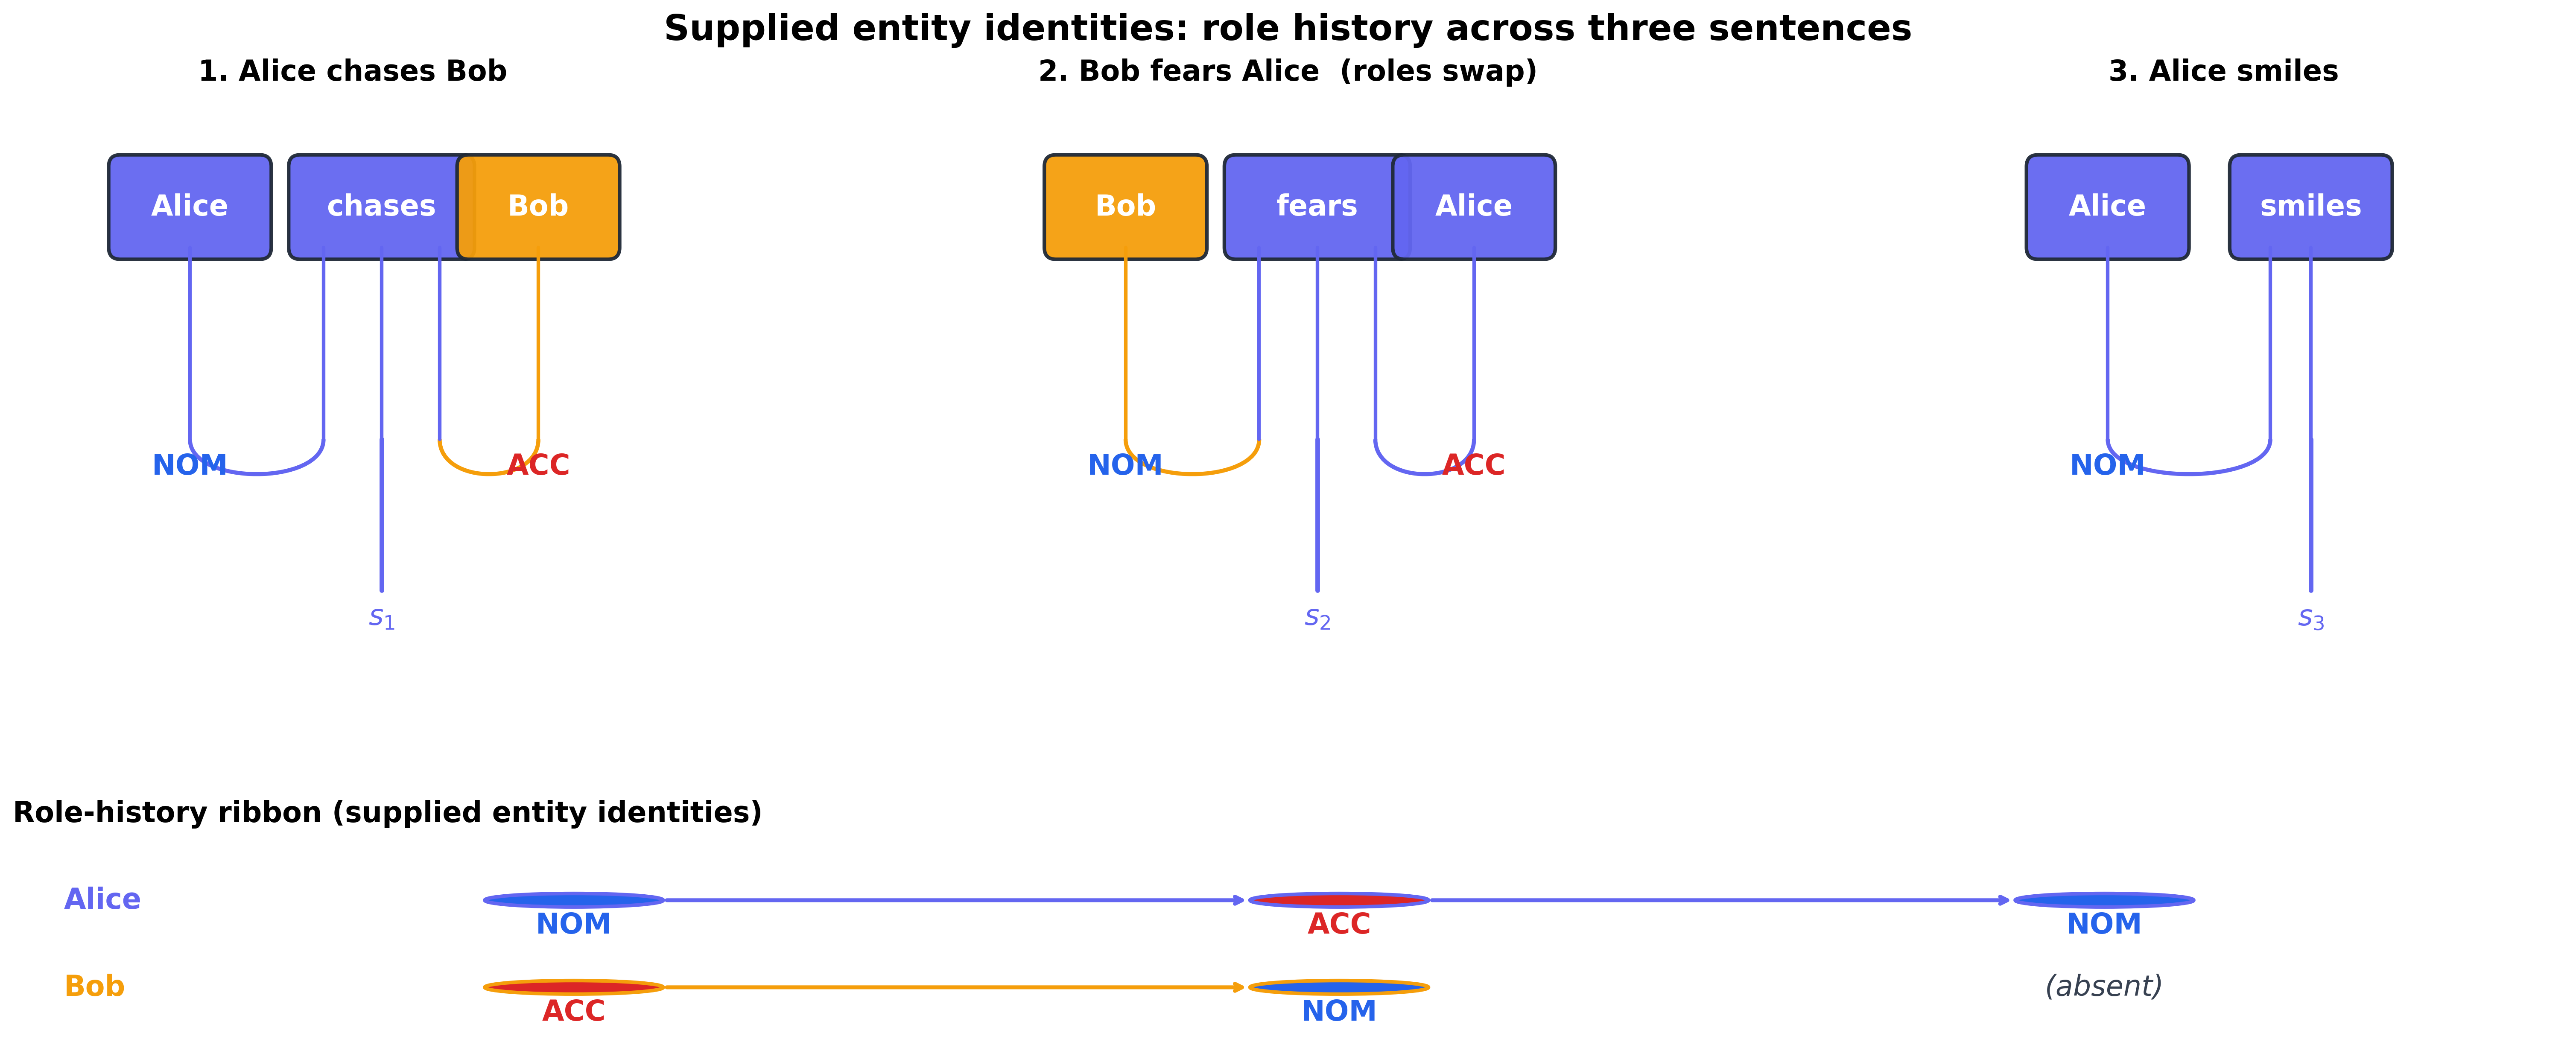
\includegraphics[keepaspectratio,alt={DisCoCirc entity-persistence unpacking for Alice chases Bob. Bob fears Alice. Alice smiles. Three sentence panels (top) plus a role-history ribbon (bottom). Each entity has a dedicated colour (Alice indigo, Bob amber) and the cup contractions are coloured by the entity each one consumes. The ribbon shows Alice traversing NOM→ACC→NOM and Bob traversing ACC→NOM (with an ``absent'' marker for sentence 3), exhibiting graphically the Frobenius-spider entity persistence that motivates DisCoCirc. Generated programmatically from src.visualization.category\_unpacking.render\_discocirc\_entity\_persistence().}]{../figures/discocirc_entity_persistence.png}}
\caption{DisCoCirc entity-persistence unpacking for \emph{Alice chases
Bob. Bob fears Alice. Alice smiles.} Three sentence panels (top) plus a
role-history ribbon (bottom). Each entity has a dedicated colour (Alice
indigo, Bob amber) and the cup contractions are coloured by the entity
each one consumes. The ribbon shows Alice traversing NOM→ACC→NOM and Bob
traversing ACC→NOM (with an ``absent'' marker for sentence 3),
exhibiting graphically the Frobenius-spider entity persistence that
motivates DisCoCirc. Generated programmatically from
\protect\texttt{src.visualization.category\_unpacking.render\_discocirc\_entity\_persistence()}.}\label{fig:discocirc-persistence}
\end{figure}
\end{frame}

\begin{frame}[fragile,allowframebreaks]{lambeq Gen II Compiles DisCoCirc
Discourse Diagrams}
\protect\phantomsection\label{lambeq-gen-ii-compiles-discocirc-discourse-diagrams}
The categorical structure of DisCoCat maps naturally onto quantum
circuits: the tensor product structure of \(\mathbf{FVect}\) is
identical to the tensor product structure of \(\mathbf{Qubit}\), the
category of qubit systems. This observation underlies the \textbf{QNLP}
(Quantum Natural Language Processing) program
{[}@meichanetzidis2020qnlp{]}, which implements DisCoCat models as
parameterized quantum circuits.

The \textbf{lambeq} library {[}@lorenz2021lambeq{]} provides a practical
pipeline:

\begin{enumerate}
\tightlist
\item
  Parse a sentence into a pregroup derivation (via the neural CCG parser
  Bobcat or rule-based parsers)
\item
  Convert the derivation into a string diagram
\item
  Translate the diagram into a parameterized quantum circuit (or a
  classical tensor network)
\item
  Train the parameters on NLP tasks (classification, similarity,
  question answering)
\end{enumerate}

Kartsaklis et al. {[}-@kartsaklis2021functorial{]} demonstrate that this
pipeline achieves competitive performance on question-answering tasks,
confirming that the categorical structure captures genuine linguistic
regularities even when instantiated on noisy near-term quantum hardware.

\textbf{lambeq Gen II} (released May 21, 2025 by Quantinuum) marks a
significant advance by incorporating full \textbf{DisCoCirc} support as
its core mathematical foundation, enabling the framework to scale beyond
single-sentence semantics to discourse-level NLP {[}@lambeq2025genii;
@quantinuum2025genii{]}. With over 50,000 downloads, lambeq Gen II
achieves language neutrality, improved trainability, and compositional
interpretability for explainable AI on quantum hardware. The new
\texttt{DisCoCircReader} API automatically compiles long texts and
multi-page documents into discourse-level quantum circuits, with entity
wires tracking semantic state persistence across sentence
boundaries---closing the gap between sentence-level DisCoCat and
discourse-level case role tracking. This is directly relevant to the
case role reversal phenomena discussed in
\autoref{fig:three-sentence-discourse}: lambeq Gen II can, in principle,
compile such multi-sentence case-dynamic discourses into trainable
quantum circuits.

Foundational work by Meyer and Lewis integrates DisCoCat with density
matrices for modeling dynamic meaning and lexical ambiguity in text,
treating semantic states as mixed quantum states---providing an
alternative to pure-state vector models that naturally accommodates
ambiguity and partial information {[}-@meyer2020modelling{]}.

Recent work on \textbf{string diagram rewriting} by Bonchi et al.
{[}-@bonchi2022rewriting{]} provides the theoretical foundation for
diagram simplification, showing that string diagram rewrite systems
modulo Frobenius structure can be interpreted as double-pushout
hypergraph rewriting---ensuring that the algebraic simplifications
applied during normal form computation are provably sound. De Huybrecht
{[}-@dehuybrecht2024subcategorizing{]} extends DisCoCat with
\emph{subcategorization} for light verb constructions, demonstrating
that the categorical framework accommodates sublexical compositional
structure---a development that connects naturally to the monadic root
syntax of Song {[}-@song2022act{]} discussed in
\autoref{sec:categorial-grammar}.

For our case-theoretic framework, QNLP offers a concrete computational
substrate: case categories could be implemented as quantum circuits
where case roles correspond to quantum registers and grammatical
relations correspond to parameterized gates. This connection between
linguistic case structure and quantum information processing---mediated
entirely by the shared categorical formalism---illustrates the power of
the diagrammatic approach.
\end{frame}

\begin{frame}[allowframebreaks]{No Barren Plateau for Local Observables}
\protect\phantomsection\label{no-barren-plateau-for-local-observables}
A central challenge for practical QNLP on near-term quantum hardware is
the \emph{trainability} of parameterized quantum circuits (PQCs): the
vanishing gradient problem, or \emph{barren plateau}, makes
gradient-based optimization exponentially hard as circuit width and
depth scale. Two recent results (2024) directly resolve this obstacle
for linguistically motivated circuits:

\begin{enumerate}
\item
  \textbf{Rad et al. {[}-@rad2024trainability{]}} introduce
  \emph{reduced-domain parameter initialization}: rather than sampling
  all parameters uniformly from \([0, 2\pi)\), one initializes the
  circuit in a small-angle domain close to the identity. For circuits of
  the depth typical of DisCoCirc discourse diagrams (compiled from
  multi-sentence texts via coreference resolution), this initialization
  provably yields polynomial rather than exponential gradient
  decay---keeping optimization tractable as discourse length grows.
\item
  \textbf{Letcher et al. {[}-@letcher2024tight{]}} derive tight,
  \emph{assumption-free} lower bounds on the variance of cost function
  gradients for PQCs with local observables (e.g., Pauli operators
  restricted to a few-qubit subsystem). Their key finding is that, for
  POVMs restricted to local observables---exactly the structure of the
  case-role measurement operators \(E_c\) of \autoref{eq:eq-8-1}
  (formalized in \autoref{sec:quantum-semantics})---no barren plateau
  effect occurs. This provides a theoretical guarantee that case-role
  classification circuits implemented via lambeq remain optimizable
  regardless of total circuit size, so long as the readout observable is
  local.
\end{enumerate}

Together, these results underpin the practical feasibility of the F1 and
F3 research directions of \autoref{sec:conclusion}: scaling case-marked
DisCoCat/DisCoCirc models to corpora-scale quantum hardware without
exponential gradient overhead. The geometric structure of lambeq's IQP
and Sim4 ansätze, combined with these initialization and observable
choices, provides a principled recipe for quantum case category training
on near-term devices.

\newpage
\end{frame}

\end{document}
